\subsection{Resultados obtenidos por el prototipo a 0.00 C}

\begin{figure}[H]
	\centering
	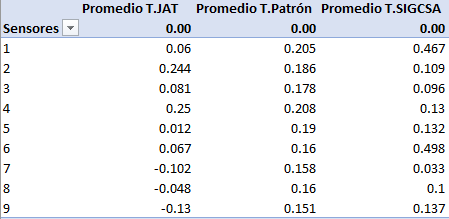
\includegraphics[width=0.5\linewidth]{resultados3.png}
	\caption{Tabla de Promedios de Temperaturas de prototipo y termómetros a 0.00 C}
\end{figure}

\par \noindent 
Los resultados obtenidos por las calibraciones, ver Anexo 4 , son utilizados para calcular la temperatura promedio del termómetro patrón, los nueve termómetros de campo de SIGCSA y los sensores de temperatura del prototipo, ver figura 4.3 y con estos valores podemos realizar la siguiente gráfica:

\begin{figure}[H]
	\centering
	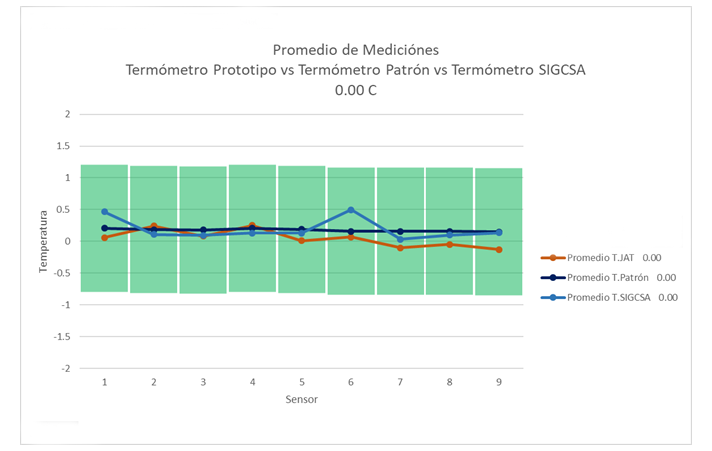
\includegraphics[width=0.6\linewidth]{resultados4.png}
	\caption{Grafica de Promedios de Temperaturas de prototipo y termómetros a 0.00 C}
\end{figure}

\par \noindent
Nuevamente los sensores del prototipo y los termómetros de campo de SIGCSA se encuentran en el rango aceptable para la compañía. Pero si comparamos la figura 4.4 y 4.2 podemos observar que ciertos sensores del prototipo y termómetros de campo, el error de ellos se empieza a ampliar con respecto al termómetro patrón. A continuación los resultados a 10.00 grados Celsius.
